\documentclass[conference]{IEEEtran}
\IEEEoverridecommandlockouts
% The preceding line is only needed to identify funding in the first footnote. If that is unneeded, please comment it out.
\usepackage{cite}
\usepackage{amsmath,amssymb,amsfonts}
\usepackage{algorithmic}
\usepackage{graphicx}
\usepackage{textcomp}
\usepackage[table,xcdraw]{xcolor}
\def\BibTeX{{\rm B\kern-.05em{\sc i\kern-.025em b}\kern-.08em
    T\kern-.1667em\lower.7ex\hbox{E}\kern-.125emX}}
\begin{document}

\title{ConfigNVPSim: GEM5 Based Configurable NVP Simulator\\
}

\author{\IEEEauthorblockN{Gulsum Gudukbay}
\IEEEauthorblockA{\textit{Computer Science and Engineering} \\
\textit{Pennsylvania State University}\\
gxg5138@psu.edu}
\and
\IEEEauthorblockN{Sethu Jose}
\IEEEauthorblockA{\textit{Computer Science and Engineering} \\
\textit{Pennsylvania State University}\\
sxj487@psu.edu}
\and
\IEEEauthorblockN{Vineetha Govindaraj}
\IEEEauthorblockA{\textit{Computer Science and Engineering} \\
\textit{Pennsylvania State University}\\
vzg99@psu.edu}
}

\maketitle

\begin{abstract}
The demand for feature rich systems like smart phones and IOT has increased over recent years. These systems could benefit from using non-volatile processors (NVP) by providing an optimal power budget along with increased performance. ConfigNVPSim, a non-volatile simulator on a gem5 platform, provides a solution to realizing a non-volatile simulator. NVP systems ensures forward progress even at intermittent energy levels. ConfigNVP system aims at improving NVPSim \cite{b1} system by adding configurability at all levels. ConfigNVP system implements new power levels to CPU based on the system energy level. Energy management unit in ConfigNVPSim monitors the system energy. The state machine implemented in the energy management unit ensures that the power levels are are switched between off, on and power retention states based on preconfigured energy thresholds. This implementation of ConfigNVPSim can be modified in future revisions to add backup and restore mechanisms to different system modules like DRAM and caches.   
\end{abstract}
\vspace{5 mm}
\begin{IEEEkeywords}
Non Volatile Processors, GEM5, Energy profiling, State Machine, Energy Harvesting, Computer Architecture, Intermittent Power Supply, Capacitor, Power Failure
\end{IEEEkeywords}

\section{ \textbf{Introduction}}
Non-Volatile Processors(NVPs) are designed to preserve the system state during power deficiencies. NVPs hide data backup and restoration from the executing software to provide an execution mode that will  eventually complete the current task. NVPs are a promising solution for energy-harvesting scenarios. The power supply in such systems are unstable and intermittent. Such systems should harvest their energy from solar, thermal or other intermittent power sources. NVPs are highly suited for such systems because of its ability to ensure that even short periods of sufficient power can help to gain forward progress. 
\subsection{NVP Architecture Overview}
 Many architectural explorations for NVPs have been previously made. There have been theoretical observations on the plausible architectures like a Non-Volatile Cache / Non-Volatile DRAM etc. But power and cost overhead to realize such a system has proved to be a major drawback. Ma et.al. investigated various designs for nonvolatile processors with different microarchitectures and different input power sources to maximize the forward progress of NVPs [need to cite]. The focus of their design was to implement different policies for backing up registers in NVPs. As mentioned, high write energy and latency overhead will be induced due to the characteristics of NVMs. Thus, cache design proves to be a significant component is nonvolatile processors as the performance gap between cores and memories increases. The NVPSim developed by Yizi Gu et. al is an efficient solution in implementing NVP simulators. The ConfigNVPSim is based on this implementation. The special focus of this project is on adding configurability to NVPSim implementation by Yizi Gu et. al \cite{b1}. This system considers the delay incurred by non-volatile components of the system and provides an approximate performance estimate.
 \subsection{Simulation Overview}
 Since NVPs have a considerable overhead in terms of its architecture, need for simulating such a system is paramount to understand its efficiency. GEM5 was used in this project the simulation platform to realize the NVP architecture. GEM5 simulator has been used for analyzing the CPU and memory-centric designs, and models for several IPs to collectively study their impact on system-level performance and power. Extra modules are implemented on GEM5 base system to make the system capable of making forward progress with an intermittent power source. This is achieved using discrete energy input which is fed at a preconfigured constant time interval to the system. Based on this, a system model which can handle such variations in power and analyze the performance was developed. The main logic behind handling the intermittent energy source is the energy management unit. This unit lets the system know when to back up the data and when to restore. Energy management unit interacts with the system CPU to communicate the power level of the input. Based on that, CPU decides on how to process the instructions to avoid any data loss.
 
\vspace{5 mm}

The goal of this paper is twofold. First is the architectural implementation of NVP on the GEM5 platform. Second, the evaluation of different configurations that can be achieved using the existing architectural implementation. 
\vspace{5 mm}

The simulated architecture offers the following features provided by NVPSim \cite{b1}:\newline
1. A simple ARM base system clocked at 100MHz
2. Energy harvester to harvest energy for the system which loads tick level energy values from a file for configurability
3. Power levels for the system which is monitored by the energy management unit. These power levels and their possible transitions are as follows:
\begin{description}
  \item[$\bullet$] POWER\_RET to POWER\_ON
  \item[$\bullet$] POWER\_ON to POWER\_RET
  \item[$\bullet$] POWER\_OFF to POWER\_ON
\end{description}
4. Addition of Energy ports to GEM5's SimObjects to communicate energy consumption levels and state changes between GEM5 modules and the energy management unit.
5. Modifications to GEM5's AtomicSimple CPU module which will switch power states based on the energy messages from the state machine

\section{\textbf{System Configuration}}
In GEM5, a python configuration file is used to build and configure the system that has to be simulated. To configure a non volatile system, a single ARM core was used and its main memory and caches as shown in Figure ~\ref{fig:basic_block}. An atomic simple model of the CPU with 100MHz CPU clock and 512MB of addressable memory range was utilized. 

\begin{figure}[htbp]
\centerline{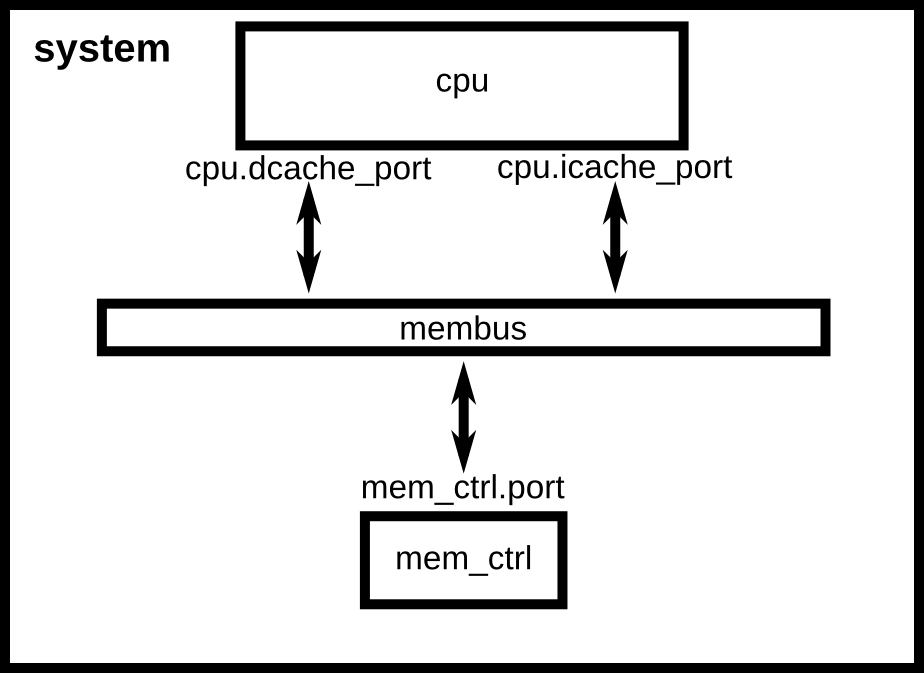
\includegraphics[scale=0.85]{simple_config.png}}
\caption{GEM5 base system configuration}
\label{fig:basic_block}
\end{figure}

In order to add the non-volatility to the system, an energy management system which updates and monitors the system's energy storage was added. The basic system configuration of~\ref{fig:basic_block} with energy harvesting module, energy manager and a state machine was augmented as shown in Figure~\ref{fig:nvpsim}. A state machine monitors the current energy level of the system and commands the system to switch between various power levels. The details of these individual modules are explained in the subsequent sections.

\begin{figure}[htbp]
\centerline{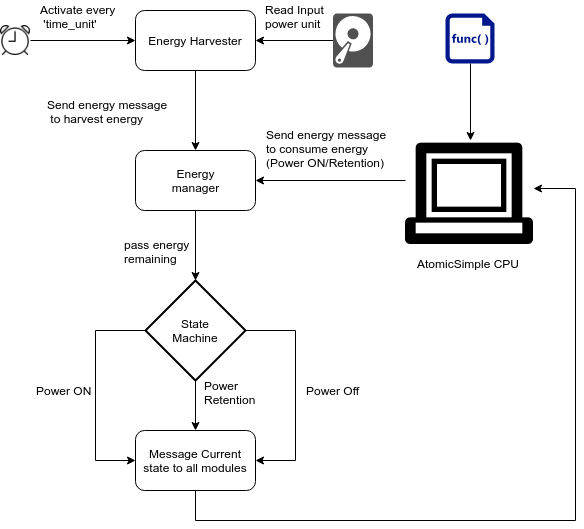
\includegraphics[scale=0.4]{nvpsim.png}}
\caption{NVPSim system}
\label{fig:nvpsim}
\end{figure}

\subsection{Energy Harvester}
The concept of an intermittent power source is not inherent to GEM5 system. To achieve better control over the input power source, input power levels can be generated using tools like Octave or Matlab. These waveforms are passed to GEM5 as an input file. To test different input conditions, the waveforms shown in Figure ~\ref{fig:sine_wave} and Figure ~\ref{fig:real_wave} were used. Figure ~\ref{fig:sine_wave} shows positive half of an ideal sine wave extended with 200 data points of 0s. This sine wave provides a simplistic input to interpret the performance of the system. Figure ~\ref{fig:real_wave} shows a real intermittent power supply. We show that NVPsim works consistently with this real world input. 

\begin{figure}[htbp]
\centerline{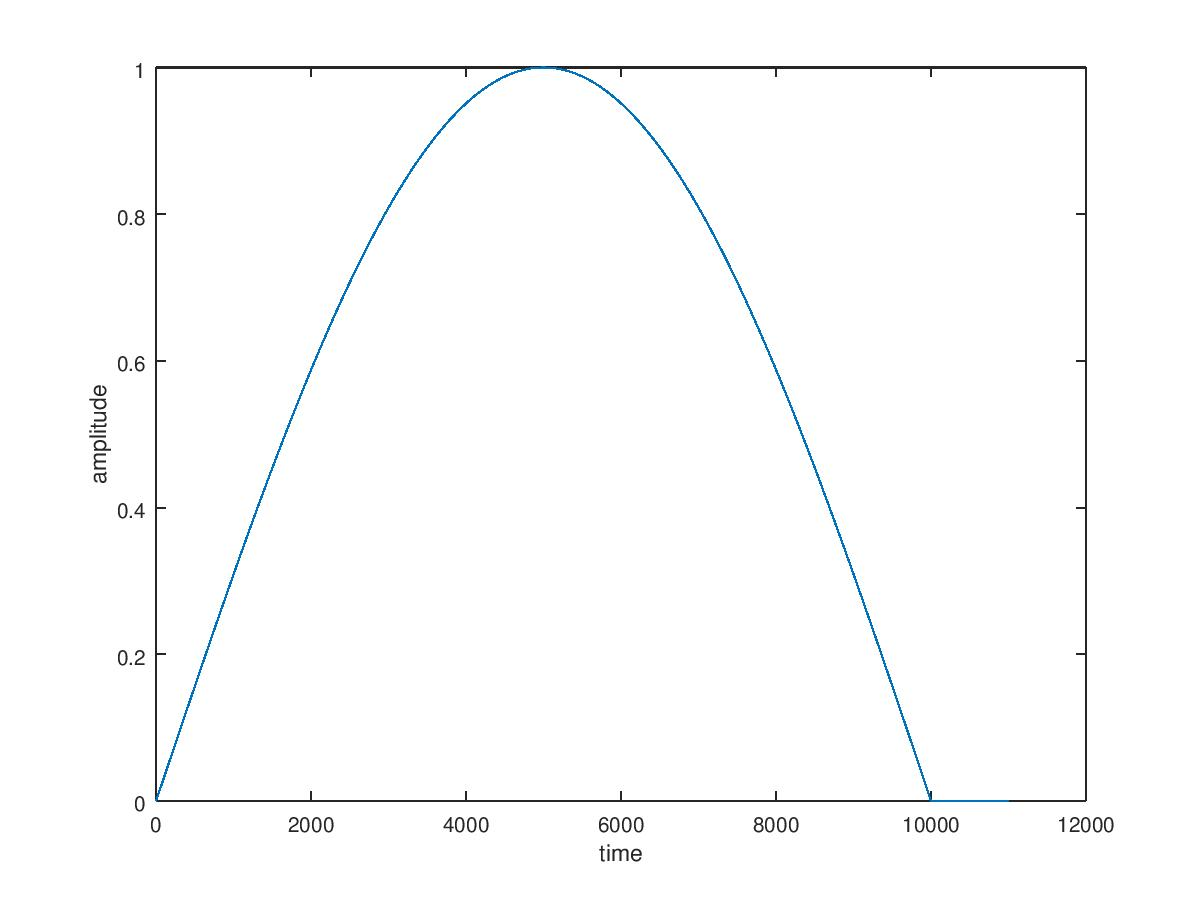
\includegraphics[scale=0.4]{sine_wave.jpg}}
\caption{Ideal Sine wave Power Source}
\label{fig:sine_wave}
\end{figure}

\begin{figure}[htbp]
\centerline{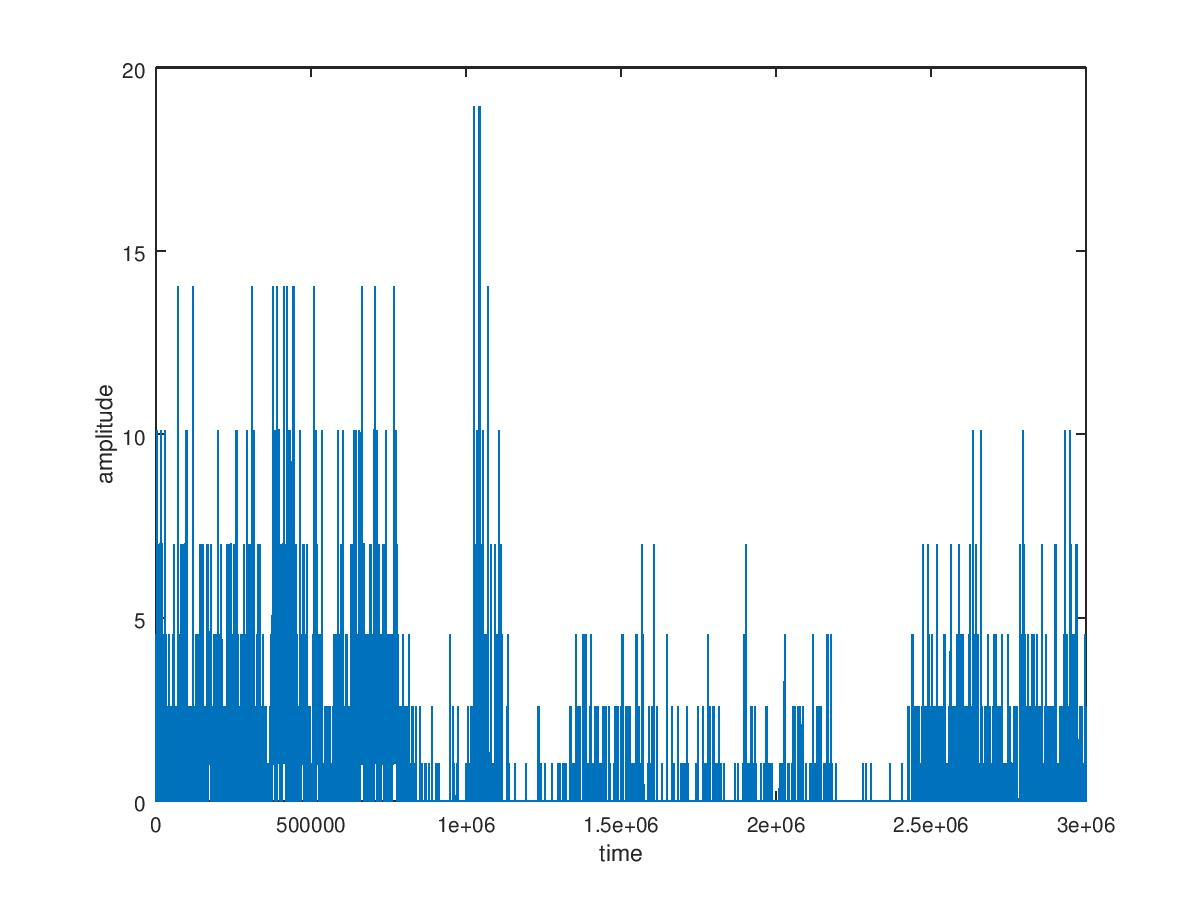
\includegraphics[scale=0.4]{real_wave.jpg}}
\caption{Real Intermittent Power Source}
\label{fig:real_wave}
\end{figure}

The python configuration file configures the energy management system with the input power file and energy consumption \textit{energy\_time\_unit} to be used in the system simulation. Upon system initialization, the energy harvester module reads and maintains a copy of the input power in the system. Then it schedules a periodic call to itself every \textit{energy\_time\_unit} interval of time to update the system energy based on the input file. Hence, \textit{energy\_time\_unit} decides at what rate the input power file is read by the energy harvester. Once the energy is read by the harvester, it updates the energy manager which maintains the current energy level of the system \textit{energy\_remained}.

\subsubsection{Energy Manager}
Energy Manager receives energy messages from energy harvester as well as the other SimObjects which consumes energy in the system. Energy harvester updates energy manager with an increase in the system energy. Other SimObjects like AtomicSimpleCPU which are consumers of energy sends messages to energy manager informing the amount of energy consumed by that individual module. Based on the source of these messages, energy manager updates the system energy. Energy manager confirms that the system energy is restricted to \textit{upper\_bound} and the \textit{lower\_bound} set in the python configuration file. Once the \textit{energy\_remained} has been successfully updated by the energy manager, it invokes the state machine module which dictates how the power level of the system should be updated. 

\subsection{State Machine}
The state machine used by the system is simple with three states - STATE\_POWER\_OFF, STATE\_POWER\_RETENTION and STATE\_POWER\_ON. The state machine state is initialized to STATE\_POWER\_OFF upon initialization. Based on the energy level information received from the energy manager module, state machine updates the states to these module. The thresholds used by the state machine to update the system is configurable through the python configuration file. When the system energy exceeds threshold \textit{thres\_ret\_to\_1}, the state machine switches the state to STATE\_POWER\_ON. The system remains in the STATE\_POWER\_ON state until, the system energy falls below  \textit{thres\_1\_to\_ret}. At this point, the state machine switches to STATE\_POWER\_RETENTION. It can remain in this state until the system energy remains above \textit{thres\_ret\_to\_off}. Once system energy falls below this threshold, the state machine switches back to STATE\_POWER\_OFF state.

The state machine uses messages to inform SimObjects regarding the state changes. The state change messages are broadcasted to all SimObjects so that they can change their power levels and functionality based on the current system energy level. When STATE\_POWER\_ON is entered, state machine sends the message POWER\_ON to all SimObjects. It sends the message POWER\_RET and POWER\_OFF when it enters the states STATE\_POWER\_RETENTION and STATE\_POWER\_OFF respectively. To implement the messaging system, the SimObject definitions were augmented with an energy port for sending and receiving these messages. 

In this implementation, only the AtomicCPU was modified to receive the energy messages broadcasted by the state machine. Moreover, AtomicCPU is the only module in ConfigNVPSim system which can consume power. Extension of energy consumption to other modules like DRAM and cache has to be updated in the subsequent release versions of ConfigNVPSim. 

\subsection{AtomicCPU}
AtomicCPU receives the energy messages from the state machine through the energy port. GEM5 keeps the CPU running by scheduling and executing ticks at CPU clock periods. CPU ticks can be controlled to stop or to pause the CPU execution. This strategy is adopted in NVP system to implement non-volatility. 
When the AtomicCPU receives a state change message to POWER\_OFF, the CPU enters the POWER\_OFF state by descheduling the previously scheduled tick. This ensures that the CPU doesn't run anymore and that it is powered off. When state machine switches the CPU state to POWER\_RET state, the CPU ticks are rescheduled to the subsequent tick period which prevents the CPU execution. The tick rescheduling continues until the next state change. When the POWER\_ON state is entered, the rescheduled and turned off tick is restored and CPU starts execution. 
When the state change is from POWER\_RET to POWER\_ON, the system remembers the previous state and tick is restored from the last backed up tick.

\section{\textbf{Experimentation}}
ConfigNVPSim's performance with an ideal sine input was evaluated in order to examine the state changes. Two parameters were variable: state change thresholds and energy consumptions in each state. Four experiments were done: the first one was with threshold settings 1 and consumption settings 1, second one was threshold settings 2 and consumption settings 1, third one was threshold settings 1 and consumption settings 2 and the last one was ConfigNVPSim's response to real power input that was fed into the base Gem5 implementation. To visually observe the state changes and energy remained in each state change,  the input power, energy remained and state was plotted in one graph for each experiment. Tables \ref{table:cpuconsumption} and \ref{table:cputhresh} show threshold settings and consumption configurations.
To test the performance of ConfigNVPSim, a program called nvp\_hello.c was executed. The functionality of this program includes a loop that increments and prints a counter. The aim of this program is to confirm that the CPU only executes programs in POWER\_ON state. 
\begin{table}[]
\medskip
\begin{center}
\begin{tabular}{|l|l|l|l|}
\hline
\rowcolor[HTML]{D9D9D9} 
Configuration & POWER\_ON & POWER\_RET & POWER\_OFF \\ \hline
1             & 0         & 0.3        & 1.3        \\ \hline
2             & 0         & 1.5        & 6.5        \\ \hline
\end{tabular}
\end{center}
\medskip
\caption{CPU Energy Consumption Configurations}
\label{table:cpuconsumption}
\end{table}

\begin{table}[]
\medskip
\begin{center}
\begin{tabular}{|l|l|l|l|}
\hline
\rowcolor[HTML]{D9D9D9} 
Configuration & POWER\_ON & POWER\_RET & POWER\_OFF \\ \hline
1             & 40        & 80         & 500        \\ \hline
2             & 200       & 400        & 1000       \\ \hline
\end{tabular}
\end{center}
\medskip
\caption{CPU State Threshold Configurations}
\label{table:cputhresh}
\end{table}

\section{\textbf{Results}}
Figure ~\ref{sine3} shows the state changes in ConfigNVPSim with threshold settings 1 and power consumption settings 1. With these settings and the positive half of the sine wave as input, it can be seen that the state changes to POWER\_RET once the system energy is depleted. Once the system energy builds back, the CPU starts executing the code. The system goes through multiple iterations of switches between POWER\_RET and POWER\_ON before the input wave dies out and system falls back to POWER\_OFF. 

\begin{figure}[htbp]
\centerline{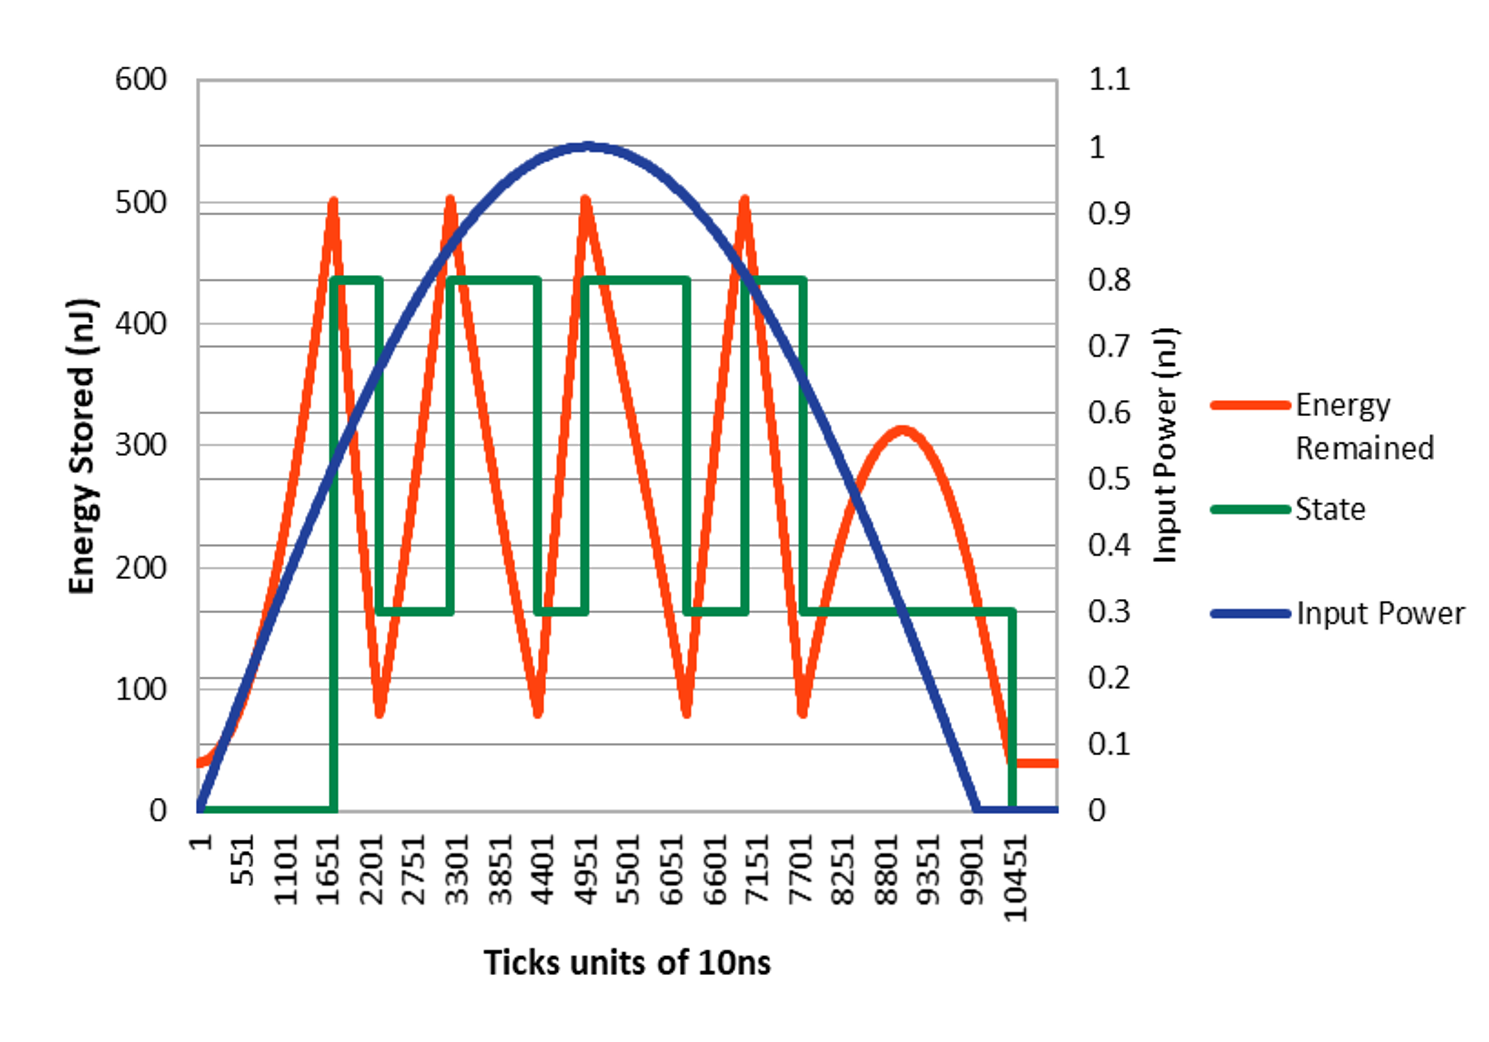
\includegraphics[scale=0.3]{sine3.png}}
\caption{Performance with sine input (threshold settings 1 and consumption settings 1)}
\label{sine3}
\end{figure}

Figure ~\ref{sinediffthresh3} shows the state changes in ConfigNVPSim with threshold settings 2 and consumption settings 1. As shown in ~\ref{table:cputhresh}, Threshold settings 2 sets the thresholds at higher energy level than Threshold settings 1. This difference is reflected in the reduction in number of state changes between POWER\_RET and POWER\_ON.

\begin{figure}[htbp]
\centerline{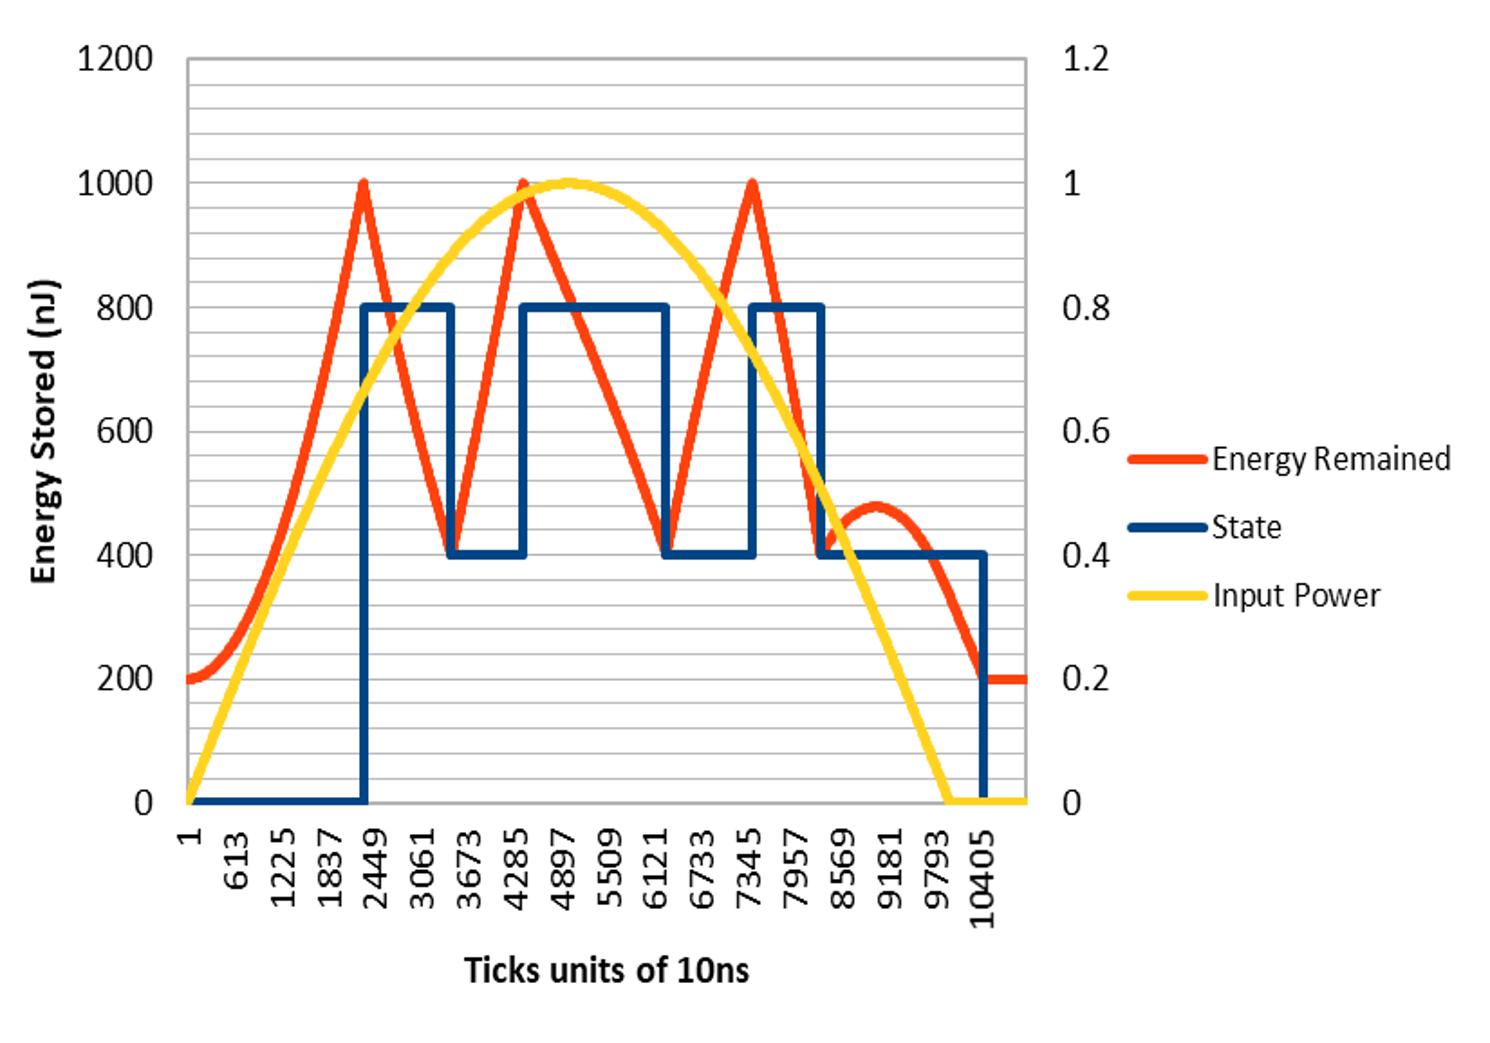
\includegraphics[scale=0.3]{sinediffthresh3.png}}
\caption{Performance with sine input (threshold settings 2 and consumption settings 1)}
\label{sinediffthresh3}
\end{figure}

Figure ~\ref{sinediffcons3} shows the state changes with threshold settings 1 and consumption settings 2. With this setting, the power consumption in POWER\_RET and POWER\_ON is higher which results in a steeper ramp down slop and higher number of switches between POWER\_RET and POWER\_ON. 

Figure ~\ref{fig:real} shows the response of NVP system to a real world intermittent energy signal. The random variations in the input signal brings unpredictability to the time duration required to complete the CPU task. This makes non-volatile system ideal for non critical or optional tasks rather than time critical tasks.

\begin{figure}[htbp]
\centerline{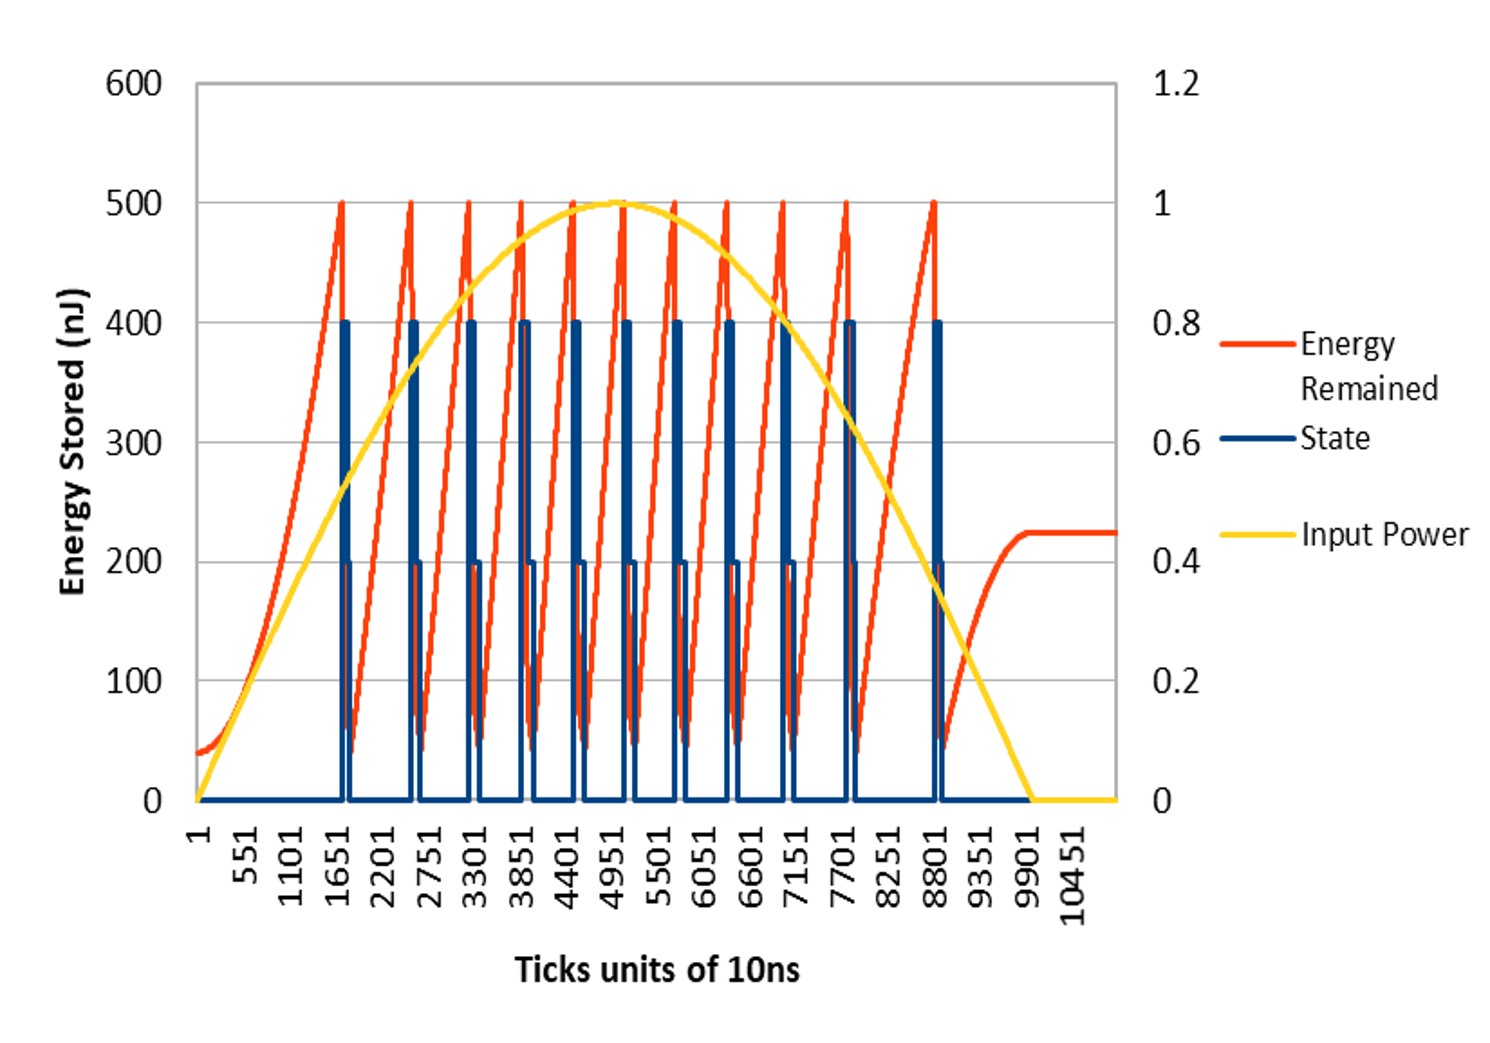
\includegraphics[scale=0.3]{sinediffcons3.png}}
\caption{Performance with sine input (threshold settings 1 and consumption settings 2)}
\label{sinediffcons3}
\end{figure}

\begin{figure}[htbp]
\centerline{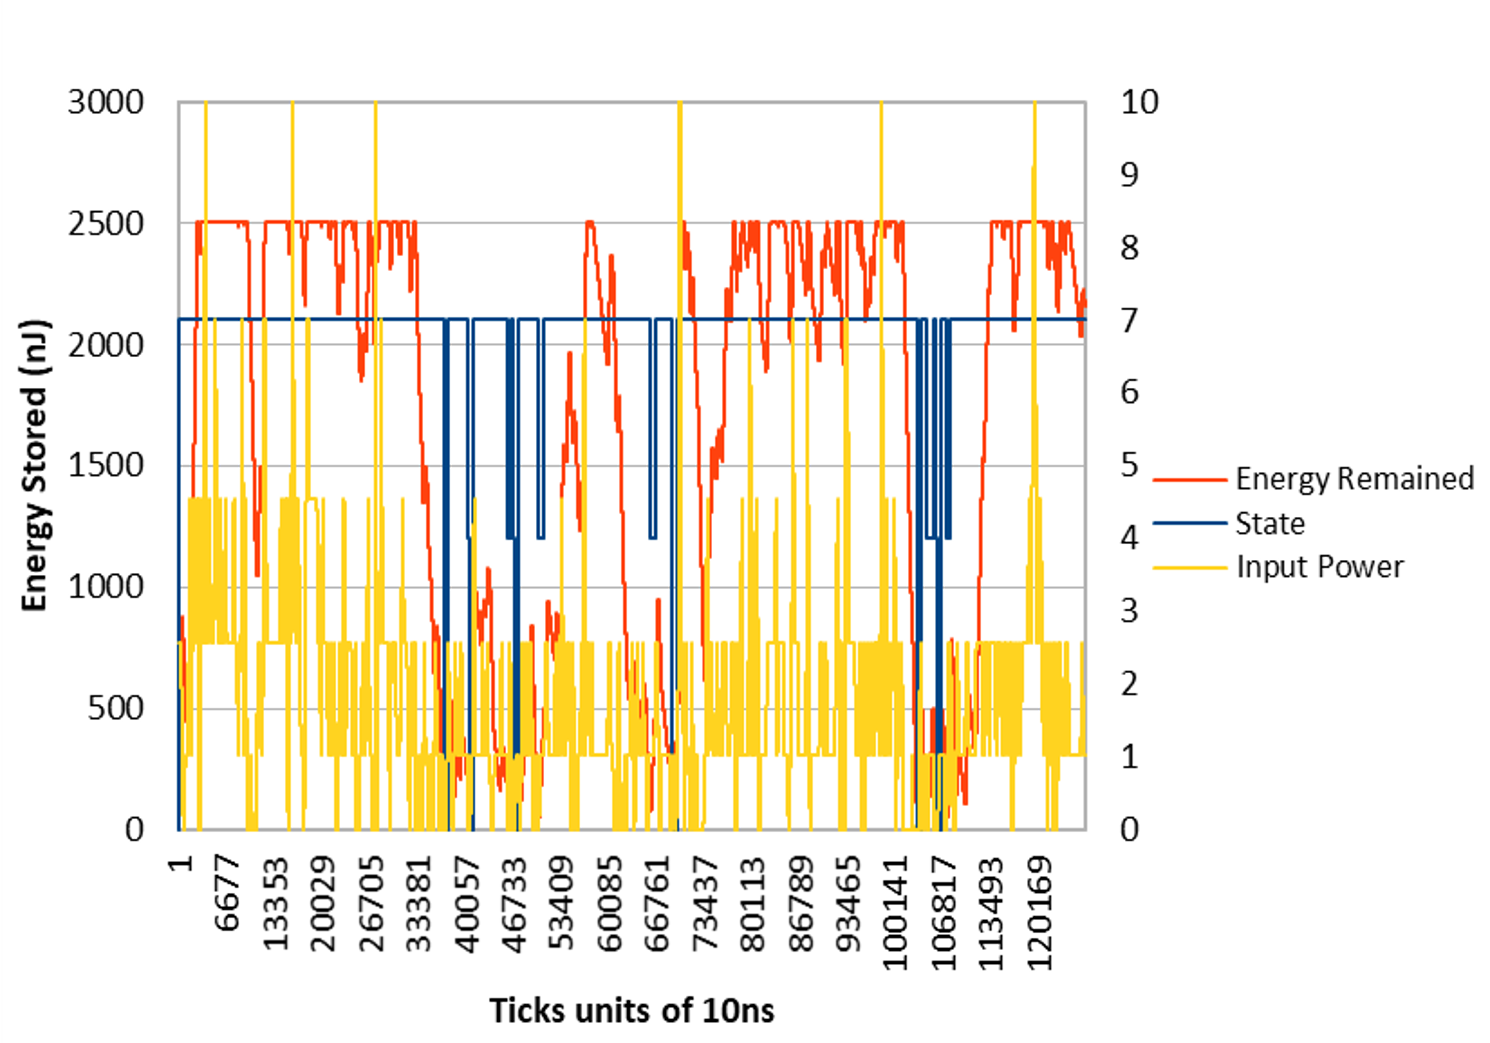
\includegraphics[scale=0.3]{orig3.png}}
\caption{ConfigNVPSim's response to real power input}
\label{fig:real}
\end{figure}

\section*{\textbf{Conclusion}}
By presenting the idea of ConfigNVPSim, the goals of implementing NVP on the GEM5 platform in terms of architecture and the evaluation of various configurations that can be created utilizing the currently existing architectural implementation were proposed. In this work, an NVP system that can maintain forward progress at intermittent energy level was created. The energy harvesting unit, state machine that controls the instantaneous energy storage of the system and lastly an AtomicCPU unit that schedules the ticks and controls the CPU's power states were the heart of ConfigNVPSim, because they were the main modifications done to the existing base GEM5 implementation to meet the proposed goals. Four experiments were done to evaluate the performance of ConfigNVPSim using different energy consumption and CPU state threshold settings. 
Even though non-volatility was successfully implemented on top of the base implementation of GEM5 in terms of energy harvesting module and a state machine that controls the CPU states, the specific module for the backup of data was not implemented in this project, so that can be implemented along with different backup strategies in future work. Since the demand for feature-rich mobile systems like smart phones and tablets has increased, NVP in such a system would provide an optimal power budget paired with increased performance. So as future work, a non-volatile simulator on an android platform would provide a promising solution to realize NVP based mobile systems. Lastly, a capacitance leakage model was not implemented in the energy management unit and should be implemented as future work, to make the simulations closer to real life situations. 

\section*{\textbf{Acknowledgment}}

This work is a derivative of the NVPSim work done by Yizi Gu et. al. so we specially thank to all the prior contributors of NVPSim and Gem5. We notably thank to Prof. Jack Sampson and Prof. Mahmut Kandemir for their guidance. We also thank to Prof. Asheesh Kolli for the support.

\begin{thebibliography}{00}
\bibitem{b1}Yizi Gu, Y. Liu, Y. Wang, H. Li and H. Yang, "NVPsim: A simulator for architecture explorations of nonvolatile processors," 2016 21st Asia and South Pacific Design Automation Conference (ASP-DAC), Macau, 2016, pp. 147-152.
\bibitem{b2}Nathan Binkert, Bradford Beckmann, Gabriel Black, Steven K. Reinhardt, Ali Saidi, Arkaprava Basu, Joel Hestness, Derek R. Hower, Tushar Krishna, Somayeh Sardashti, Rathijit Sen, Korey Sewell, Muhammad Shoaib, Nilay Vaish, Mark D. Hill, and David A. Wood. 2011. The gem5 simulator. SIGARCH Comput. Archit. News 39, 2 (August 2011), 1-7. DOI=http://dx.doi.org/10.1145/2024716.2024718
\bibitem{b3} Jason Lowe-Power, Learning Gem 5, Retrieved from http://learning.gem5.org/
\end{thebibliography}
\vspace{12pt}

\end{document}
